\section{Experimenty}

Experimenty této práce probíhaly především na počítačích uvedených v~předchozí kapitole. Nejprve je však vhodné zmínit konfiguraci daných počítačů:
\begin{itemize}
\item\textbf{HummingBoard Pro} - na tomto počítači je nainstalován Linux Debian 8.1 s~označením \uv{jessie} s~grafickým rozhraním MATE 8.
\item\textbf{Banana PI} - na tomto počítači je nainstalován Linux Debian 8.1 s~označením \uv{jessie} s~grafickým rozhraním Xfce 4.10. 
\item\textbf{Raspberry PI} - na tomto počítači je nainstalován Linux Raspbian. 
\end{itemize}
Dále pro srovnání výkonu těchto počítačů byl program otestován i~na desktopovém počítači, na kterém byl zároveň vyvíjen a~odladěn. Jeho parametry jsou následující: 
\begin{itemize}
\item\textit{Intel Core i7--6700k}, operační paměť  \textit{32 GB} a~operační systém  \textit{Windows 10 Pro}.
\end{itemize}
První sada experimentů byla detekce pomocí histogramů orientovaných gradientů a~jeho vylepšení pomocí algoritmu pro substrakci pozadí při detekci ze statických kamer.

\subsection{Nalezení optimálního klasifikátoru}

Nalezení optimálního a~spolehlivého klasifikátoru je klíčovou částí celého procesu. Zároveň se jedná o~velmi komplikovaný a~zdlouhavý úkol. Je důležité zvolit ideální trénovací sadu vzorků a~k~vzhledem zvoleného typu SVM i~také jejího jádra. Otestoval jsem varianty $C$--SVC, $\nu$--SVC, $\varepsilon$--SVR klasifikátorové typy s~lineárním a~Gaussovým jádrem, přičemž jsem zjistil, že nejlepší sestava pro detekování chodců je kombinace 
typu $\varepsilon$--SVR s~lineárním jádrem, protože úspěšnost detekce byla značně vysoká. Po zvolení správného jádra a~typu klasifikátoru je dalším krokem vybrat, jak už bylo zmíněno, trénovací sadu. Vyzkoušel jsem nejrůznější trénovací sady dostupné na internetu, a~také jejich kombinace.

Nejlepších výsledků jsem dosáhl s~pozitivní trénovací sadou Dase \cite{sudipdas}, CUHK01 campus \cite{cuhk} a~jako negativní sadu jsem použil Daimler--Mono\cite{daimler}, kterou jsem nastříhal na vzorky. Tyto sady jsou součastí přílohy této práce. Následujícím krokem je zvolení správných parametrů trénování klasifikátoru. 

Trénování klasifikátoru je velmi citlivé na tyto parametry. Při změně některého z~nich, byť jen o~tisícinu, můžeme získat úplně jiný výsledek. Trénování probíhalo dvakrát za sebou. Při druhém trénování se klasifikátor učil ze svých špatných detekcí, čemuž se říká \uv{Bootstrapping} \cite{bootstrap} a tento postup je ilustrován ve zdrojovém kódu \ref{src:double_train}.
\newpage

\begin{lstlisting}[label=src:double_train, language=cpp, caption=Bootstrapping]
		cv::Size posSize = posSamplesLst[0].size();
		cv::HOGDescriptor myHog;
		myHog.winSize = posSize;
		std::vector < cv::Rect > locations;
		std::vector < float > hogDetector;
		
		getSvmDetector(svm, hogDetector);
		myHog.setSVMDetector(hogDetector);

		std::vector < cv::Rect > detections;

		for (size_t i~= 0; i~< negSamplesLst.size(); i++)	{
			myHog.detectMultiScale(negSamplesLst[i], detections);
			for (size_t j = 0; j < detections.size(); j++)	{
				cv::Mat detection = negSamplesLst[i](detections[j]).clone();
				resize(detection, detection, posSize);
				negSamplesLst.push_back(detection);
			}
		}
		labels.clear();
		labels.assign(posSamplesLst.size(), +1);
		labels.insert(labels.end(), negSamplesLst.size(), 0);

		gradientLst.clear();
		extractFeatures(posSamplesLst, gradientLst);
		extractFeatures(negSamplesLst, gradientLst);

		convertSamples2Mat(gradientLst, trainMat);
		trainSvm(trainMat, labels);
\end{lstlisting}

Natrénoval jsem klasifikátory s~různými parametry a~otestoval je na testovacích vzorcích. Tyto vzorky byly vyextrahované obrázky chodců a~"ne-chodců" z~testovacího videa pomocí jejich anotací a~přiloženého nástroje pro tvorbu vzorků a~také z~projektu PETA \cite{peta}, konkrétně se jednalo o~sady: \textit{3DPeS, CAVIAR4REID, CBLC, SARC3D a~VIPeR}. Tento krok je v~podstatě první filtrací klasifikátorů. Vybíráme takový klasifikátor, aby jeho detekce byla co nejvíc přesná a~detekoval, co nejméně špatných oblasti. Vytrénoval jsem 15 klasifikátorů s~různými parametry trénování. Tyto klasifikátory jsem nadále filtroval pomocí ROC křivky a~vybral ten nejlepší podle veličiny AUC z~grafu, který je na obrázku \ref{fig:rocCurve1}. Nastavení trénovacích parametrů jsou uvedeny v~tabulce \ref{classTab1}. Parametry $\varepsilon$, kritéria ukončení a~počet pozitivních vzorků (5649) byly stejné.

ROC křivka je takový graf, který ilustruje schopnost a~optimalizaci binárního klasifikátoru pro všechny přípustné hodnoty prahů. Křivka je vytvořena vynesením relativní četnosti skutečně pozitivních případů (true positive rate - TPR) na svislé ose a~relativní četnosti falešně pozitivních případů (false positive rate - FPR) na ose vodorovné. Čím je plocha pod křivkou (AUC) větší, tím má klasifikátor menší chybovost. 

\begin{figure}[H]
\centering
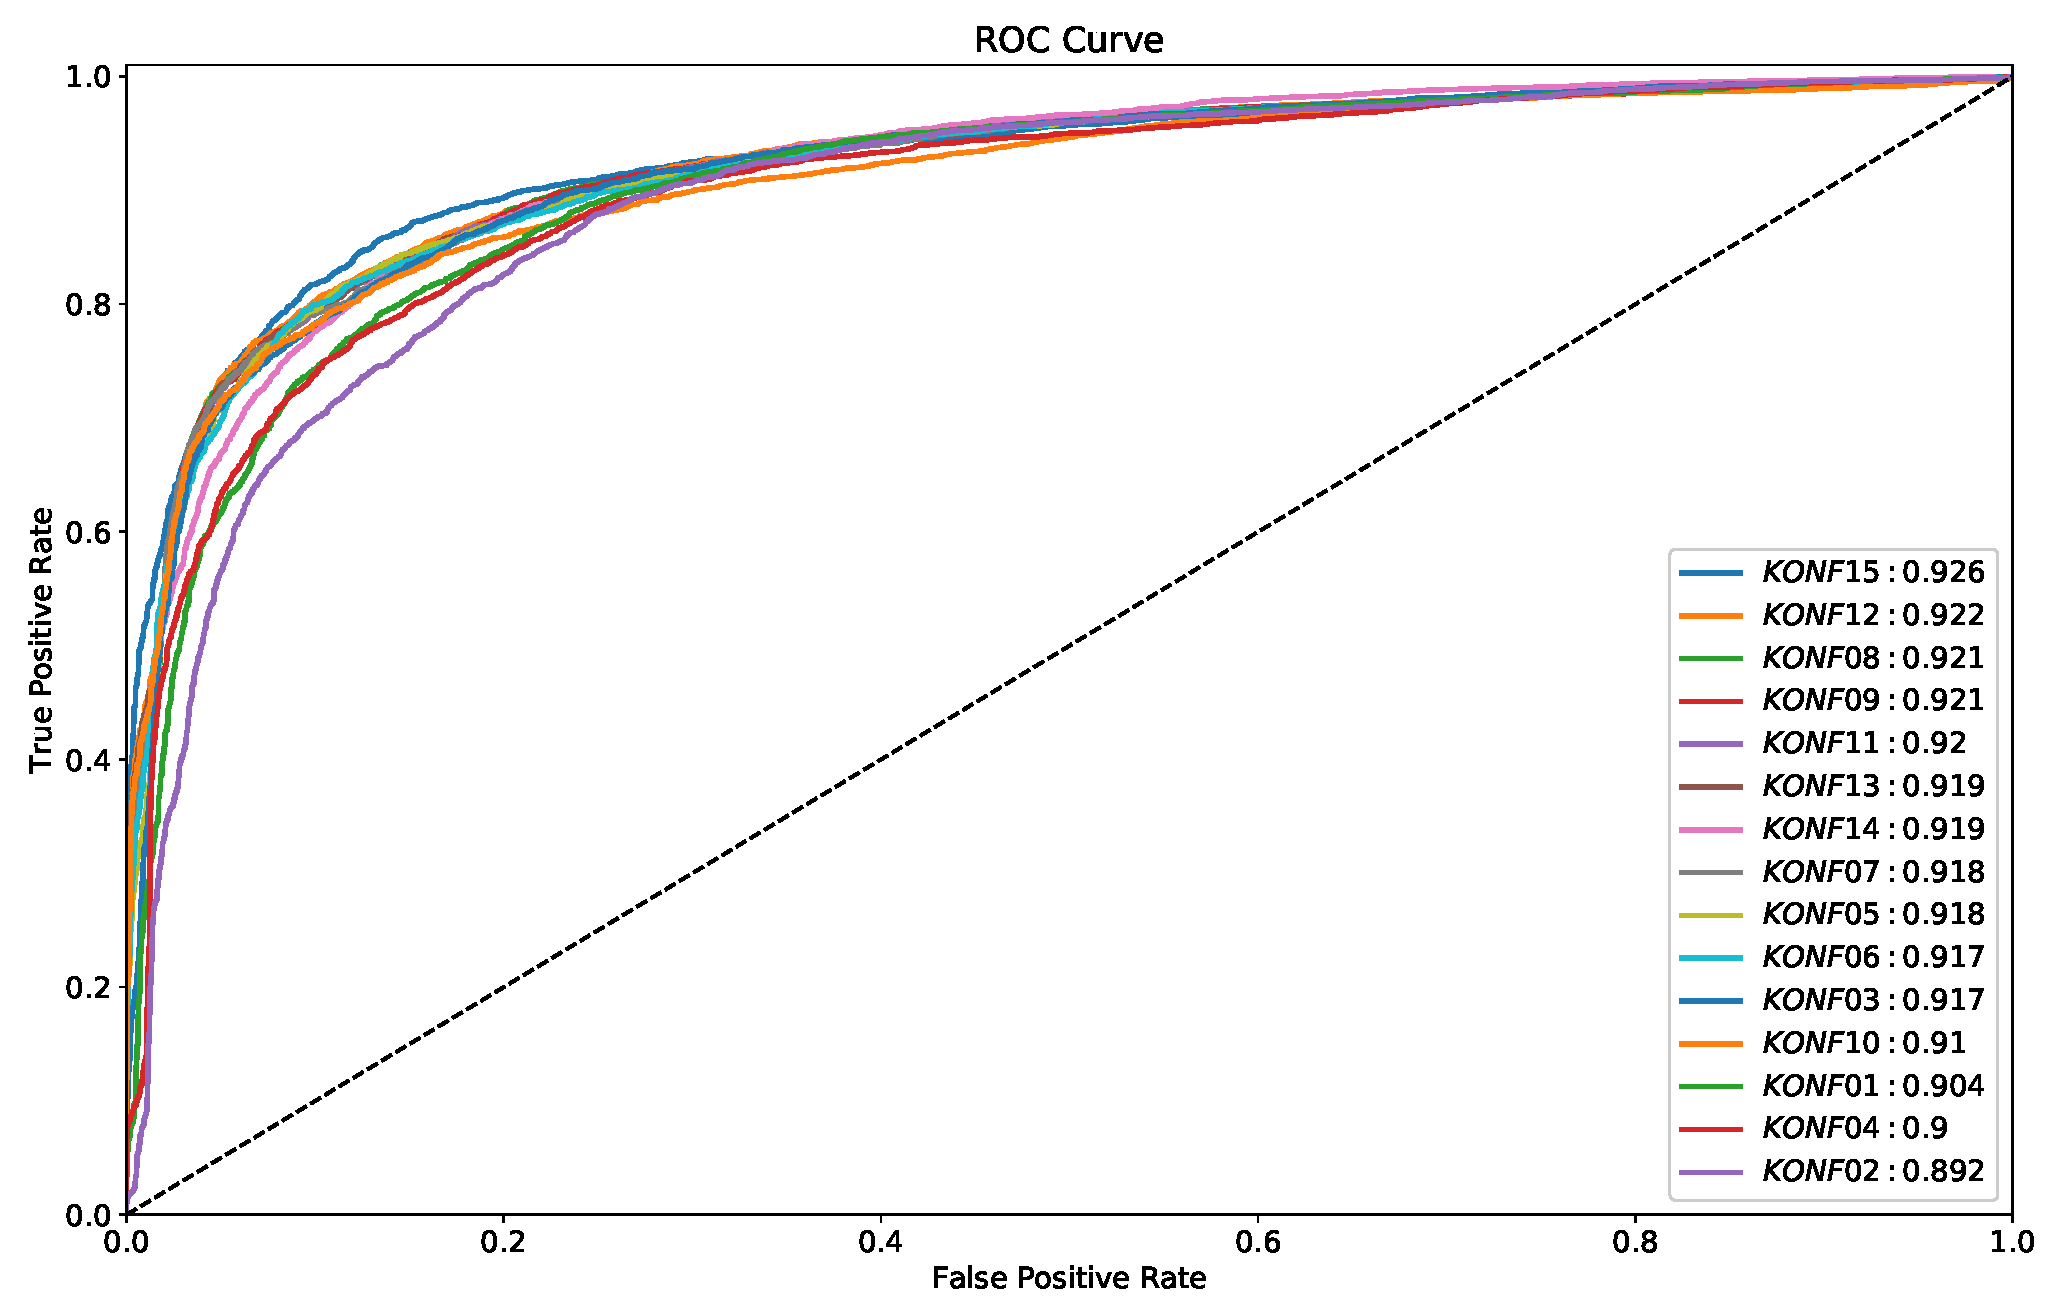
\includegraphics[width=16cm]{figures/roc1}
\caption{ROC křivka vytrénovaných klasifikátorů}
\label{fig:rocCurve1}
\end{figure}

\begin{table}[H]
\centering
\caption{Přehled vytrénovaných klasifikátorů a~jejich trénovacích parametrů.}
\begin{tabular} { |c|c|c|c|c|c| }
\hline
{Název}        & {par. C}     & {par. P}      & {max iterací} & {počet neg. vzorků} & {Přesnost \%}  \\ \hline
KONF 01		& 	0.005	& 	  0.02	 &   2000   	  &		  3000   	    &        83	 \\ \hline
KONF 02		& 	0.005	& 	  0.01	 &   3500   	  &		  3000   	    &        81	 \\ \hline
KONF 03		& 	0.001	& 	  0.02	 &   2000   	  &		  6000   	    &        83	 \\ \hline
KONF 04		& 	0.001	& 	  0.02	 &   4500   	  &		  6000   	    &        81	 \\ \hline
KONF 05		& 	0.005	& 	  0.4 	 &   3500   	  &		  6000   	    &        84	 \\ \hline
KONF 06		& 	0.01 	& 	  0.4 	 &   3000   	  &		  6000   	    &        84	 \\ \hline
KONF 07		& 	0.005	& 	  0.01	 &   2500   	  &		  9000   	    &        82	 \\ \hline
KONF 08		& 	0.005	& 	  0.25	 &   2000   	  &		  9000   	    &        82	 \\ \hline
KONF 09		& 	0.005	& 	  0.25	 &   3000   	  &		  9000   	    &        82	 \\ \hline
KONF 10 	     & 	0.01 	& 	  0.02	 &   3000   	  &		  9000   	    &        80	 \\ \hline
KONF 11 	     & 	0.01 	& 	  0.25	 &   2000   	  &		  9000   	    &        82	 \\ \hline
KONF 12 	     & 	0.01 	& 	  0.25	 &   2500   	  &		  9000   	    &        82	 \\ \hline
KONF 13 	     & 	0.01 	& 	  0.25	 &   4500   	  &		  9000   	    &        82	 \\ \hline
KONF 14 	     & 	0.5	 	& 	  0.1	 &   1200   	  &		  9000   	    &        81	 \\ \hline
KONF 15 	     & 	0.5		& 	  0.1	 &   2000   	  &		  9000   	    &        83	 \\ \hline
\end{tabular}
\label{classTab1}
\end{table}

Vybral jsem konfiguraci 15, protože oblast pod křivkou byla největší ze všech vytrénovaných. Přesnost tohoto klasifikátoru je v~tabulce \ref{classTab2}. Výsledky testování ostatních klasifikátorů jsou v~příloze této práce. Detekce může nabývat maximálně 4 stavů:
\begin{itemize}
	\item{True Positive (\textbf{TP}) - detektor správně rozpoznal chodce.}
	\item{True Negative (\textbf{TN}) - detektor tuto oblast správně ignoroval.}
	\item{False Positive (\textbf{FP}) - detektor označil tuto oblast za chodce, ovšem se ten zde nenachází.}
	\item{False Negative (\textbf{FN}) - v~oblasti se vyskytuje chodec avšak byl ignorován.}
\end{itemize}
Díky těmto stavům můžeme vypočítat přesnost detekce:
\begin{equation*}
\centering
 \label{eq:accuracy}
 \begin{aligned}
 Přesnost = \frac{TP + TN}{TP + TN + FP + FN}
 \end{aligned}
\end{equation*}

\begin{table}[H]
\centering
\caption{Přesnost konfigurace klasifikátoru číslo 15}
\begin{tabular} { |c|c|c|c|c| }
\hline
{}          & {TP/FN} 	 & {TN/FP} 	& {Přesnost \%} & {AUC}  \\ \hline
KONF 15 	  &  3479/1572  & 4912/192    &     83 		 & 0.926  \\ \hline
\end{tabular} 
\label{classTab2}
\end{table}
Na tento klasifikátor jsem se rozhodl aplikovat algoritmus substrakce pozadí, a~tak zefektivnit jeho rychlost a~správnost detekce na videosekvenci ze statické kamery.  Samotný klasifikátor byl také otestován na testovacích obrázcích ze sady \cite{testimg}. Výsledky detekce jsou na vybraných obrázcích \ref{fig:detectionExample}. V příloze \ref{appFigure} jsou umístěny další příklady.
\begin{figure}[H]
\centering
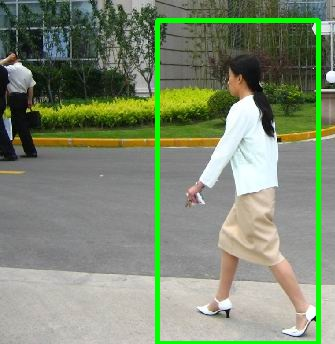
\includegraphics[keepaspectratio, max height=4cm,]{figures/ped/d1}%
\hfill % <-- Seperation
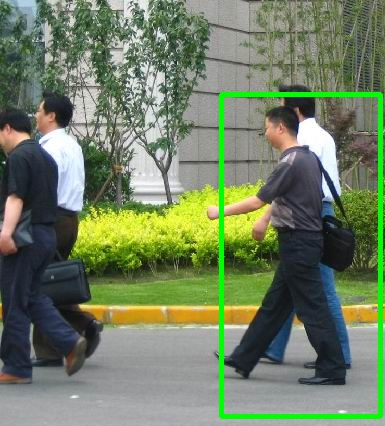
\includegraphics[keepaspectratio, max height=4cm,]{figures/ped/d2}%
\hfill % <-- Seperation
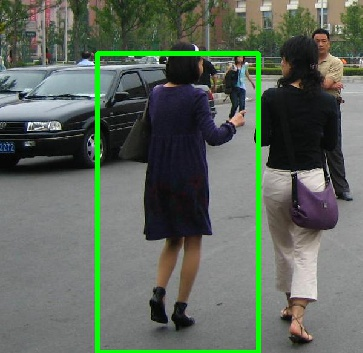
\includegraphics[keepaspectratio, max height=4cm,]{figures/ped/d3}%
\label{detectionExample2}
\end{figure}
\begin{figure}[H]
\centering
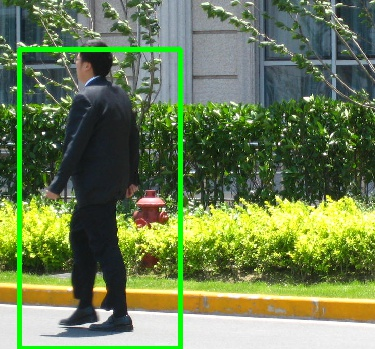
\includegraphics[keepaspectratio, max height=4cm,]{figures/ped/d4}%
\hfill % <-- Seperation
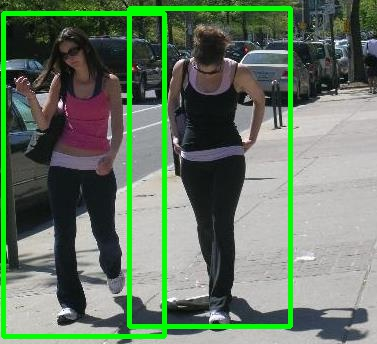
\includegraphics[keepaspectratio, max height=4cm,]{figures/ped/d5}%
\hfill % <-- Seperation
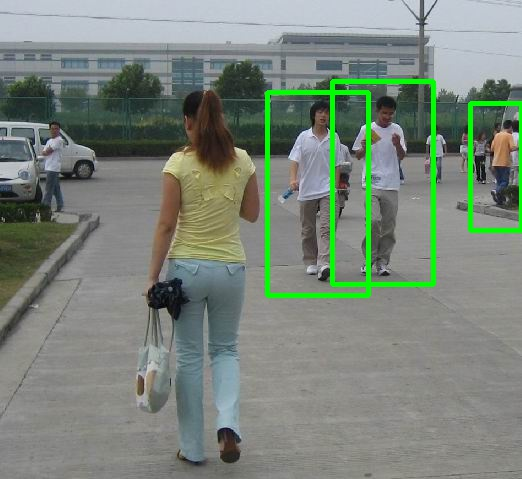
\includegraphics[keepaspectratio, max height=4cm,]{figures/ped/d6}%
\caption{Detekce na vybraných testovacích obrázcích. Obrázky jsou v~testovací sadě \cite{testimg}.}
\label{fig:detectionExample}
\end{figure}

Chodci se na obrázku mohou vyskytovat kdekoliv, proto se při takové detekci používá výpočet F1 skóre namísto přesnosti. Ke svému výpočtu totiž nepotřebuje true negative, které by bylo obtížné získat z~každého snímku. Výpočet F1 skóre je následující:
\begin{equation*}
\centering
 \label{eq:f1score}
 \begin{aligned}
F1\;  skóre = \frac{ 2TP}{2TP + FP + FN}
 \end{aligned}
\end{equation*}
Za správnou detekci je považována taková detekce, kdy výstup z~detektoru je alespoň polovina správně anotované oblasti. Příklad správné a~chybné detekce je na obrázku \ref{fig:AnotationExample}.

\begin{figure}[H]
\centering
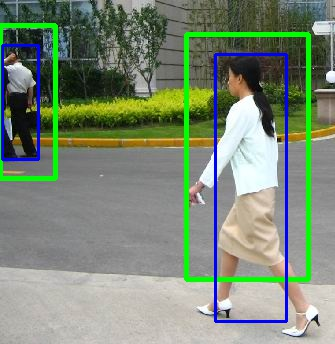
\includegraphics[keepaspectratio, max height=5.7cm,]{figures/ped/1}%
\hfill % <-- Seperation
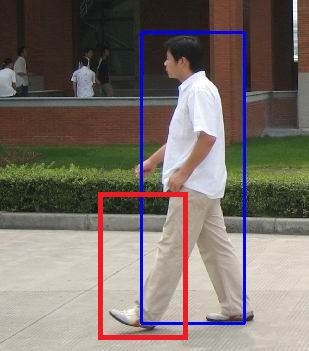
\includegraphics[keepaspectratio, max height=5.7cm,]{figures/ped/2}%
\hfill % <-- Seperation
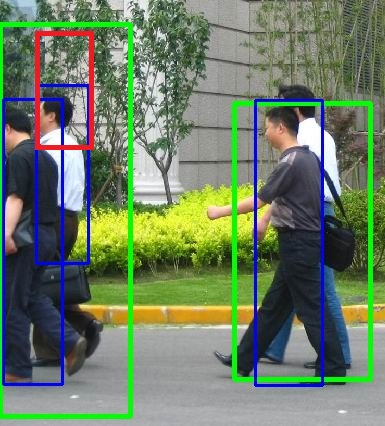
\includegraphics[keepaspectratio, max height=5.7cm,]{figures/ped/3}%
\caption{Příklady správné (zelené) a~chybné (červené) detekce. Modré obdélníky značí anotovanou oblast. Obrázky jsou v~testovací sadě \cite{testimg}.}
\label{fig:AnotationExample}
\end{figure}


\subsection{Aplikace algoritmu Mixtura Gaussiánů}
V~předchozí kapitole jsem popsal, jak probíhalo zvolení optimálního klasifikátoru a~nyní jej použijeme v~kombinaci s metodou substrakce pozadí.
Detektor nemusí procházet celý obraz, ale soustředí se pouze na vyextrahované části z obrazu. Kombinace metod HOG a~MOG může mít významný vliv na výkon celé detekce. Metoda MOG extrahuje celé dynamické popředí, to znamená, že do detektoru se nemusí dostat jenom chodec. Příklad tohoto případu zobrazuje výstupní obrázek \ref{fig:mogExample1} metody MOG, kde po extrahování popředí a aplikací eroze a dilatace zůstaly dvě významné oblasti. Tyto dvě oblasti jsou na obrázcích \ref{fig:mogExample2}. Na obrázku vlevo se nachází hledaný chodec, zatímco na pravém nikoliv. Detekce je spuštěna na obou oblastech, kde chodec byl úspěšně nalezen a druhý výřez byl ignorován. Výsledek detekce je na obrázku \ref{fig:mogExample3}.
\begin{figure}[H]
\centering
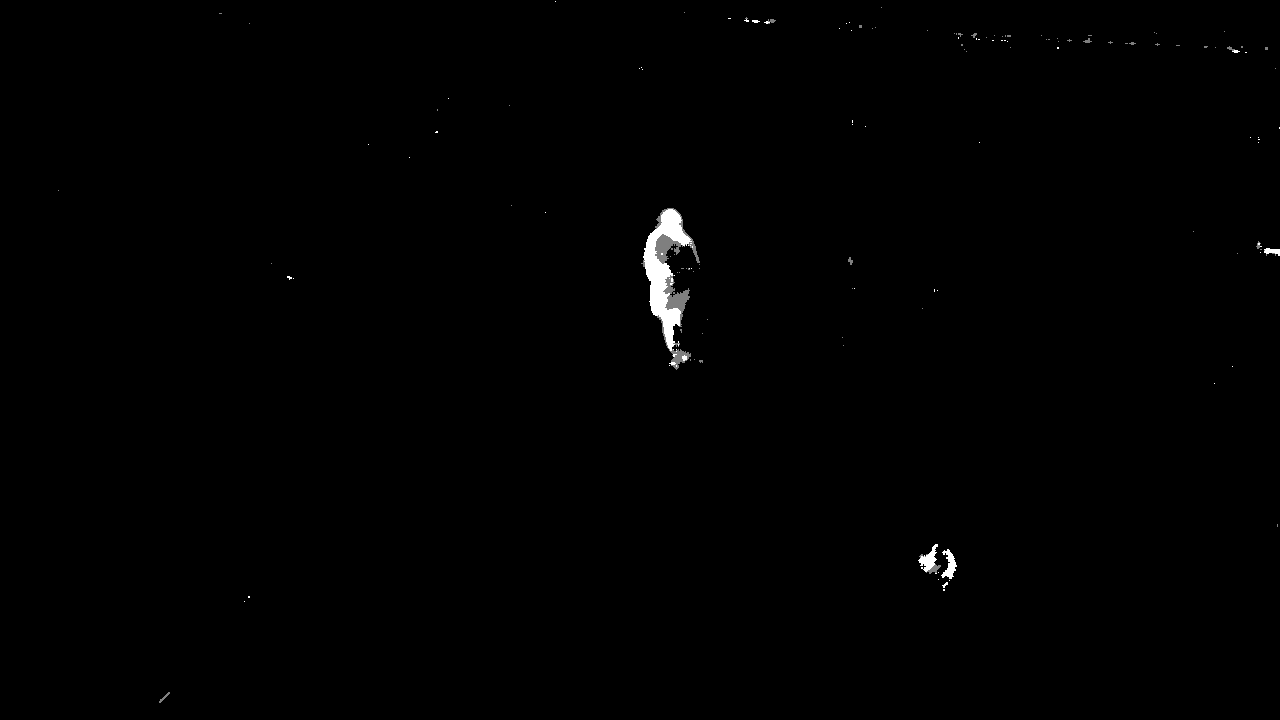
\includegraphics[keepaspectratio, max height=7.6cm,]{figures/mog/mog}%
\caption{Výstupní obrázek z metody MOG.}
\label{fig:mogExample1}
\end{figure}
\begin{figure}[H]
\centering
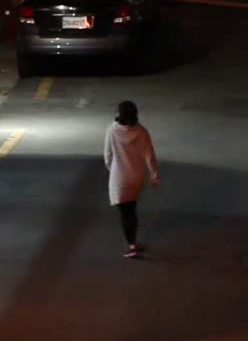
\includegraphics[keepaspectratio, max height=5cm,]{figures/mog/2}%
\vspace{0.0001cm}
\centering
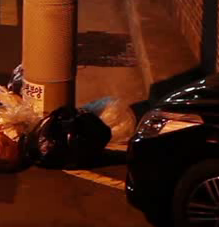
\includegraphics[keepaspectratio, max height=5cm,]{figures/mog/1}%
\caption{Výřezy z původního obrázku, na kterých je spuštěna detekce.}
\label{fig:mogExample2}
\end{figure}
\begin{figure}[H]
\centering
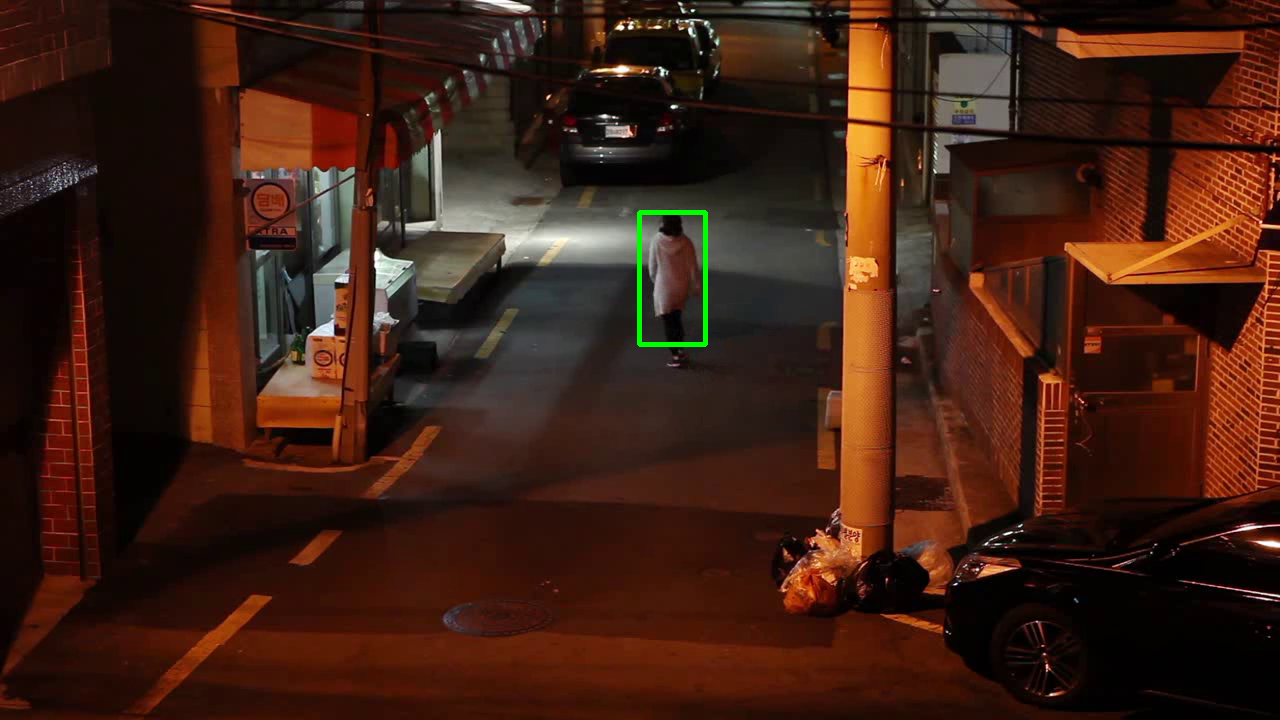
\includegraphics[keepaspectratio, max height=7.6cm,]{figures/mog/detect}%
\caption{Výsledná detekce, klasifikátor se rozhodnul správně.}
\label{fig:mogExample3}
\end{figure}
Testovací video \cite{testvideo} je ve 3 různých rozlišeních, základní informace o~videosekvencích je uvedena v~tabulce \ref{videosTab}.
Chodci v~použitých videosekvencích a~obrázcích jsou anotováni v~textových souborech.
\begin{table}[H]
\centering
\caption{Přehled testovaných videozáznamů}
\begin{tabular} { |c|c|c|c|c| }
\hline
{Název videa}   & {Rozlišení} 	     &  {Počet snímků} & {FPS} & {Výskyt osob na snímcích} \\ \hline
cctv4\_640 	 &  $640\times360$	     &      781	   & 29,97 & 	      749			    \\ \hline
cctv4\_1280	 & $1280\times720$       &      781	   & 29,97 & 	      749			    \\ \hline
cctv4\_1920 	 & $1920\times1080$	     &      781	   & 29,97 & 	      749			    \\ \hline
\end{tabular}
\label{videosTab}
\end{table}

V~tabulkách \ref{resultTabIMX}, \ref{resultTabRPI3} a~\ref{resultTabBPI} jsou uvedeny výsledky detekce z~každého videa na jednotlivém zařízení. Tabulka \ref{resultTabDesktop} znázorňuje výsledky detekce z~desktopového počítače, které slouží jako referenční model k~výsledkům výše zmíněných tabulek.  
Jsou zde také uvedeny výsledky detektoru z~knihovny Dlib (v~tabulce jako \uv{FHOG}) včetně původního detektoru lidí, který je součástí knihovny OpenCV (v~tabulce jako \uv{default HOG}) a~slouží k~porovnání s~vytrénovaným SVM klasifikátorem. Dlib klasifikátor byl vytrénován podle příkladu uvedeného na webové stránce knihovny. 
Navzdory tomu, že tyto počítače podporují rozšíření NEON a~obě knihovny byly zkompilovány s~tímto rozšířením, výsledky nebyly tak časově uspokojivé, jak jsem očekával. 
\begin{table}[H]
\catcode`\-=12
\centering
\caption{Výsledky detekce počítače HummingBoard Pro i.MX6 }
\label{resultTabIMX}
\begin{tabular}{|c|c|c|c|c|c|c|c|}
\hline
{Název videa}        & Typ algoritmu  & FPS & Délka detekce[s] & TP           & FN      & FP      & F1skóre[\%] \\  \hline
\multirow{6}{*}{cctv4\_640}  & HOG &    0,9 & 838,82  & 447 &      302 &     171 &   65,34      \\ \cline{2-8}  
      & HOG + MOG                  &    4,4 & 176,65  & 576 &    173 &     19 &      85,71      \\ \cline{2-8}  
      & FHOG                       &    1,9 & 404,41  & 238 &    511 &     43 &      46,21      \\ \cline{2-8}  
      & FHOG + MOG                 &    \textbf{5,8} & \textbf{134,10}   & 347 &    402 &     0 &       63,32      \\ \cline{2-8} 
      &  default HOG               &    0,9 & 867,73  & 299 &    450 &     24 &      55,78      \\ \cline{2-8}  
      &  default HOG + MOG         &    2,6 & 306,13  & 364 &    385 &     3 &       65,23      \\ \hline \hline   
\multirow{6}{*}{cctv4\_1280}& HOG   &    0,6 & 1 270,89  & 492 &    257 &     10 &      78,66      \\ \cline{2-8}  
      & HOG + HOG                  &    1,2 & 649,33  & 606 &    143 &     25 &      \textbf{87,83}      \\ \cline{2-8}  
      & FHOG                       &    0,5 & 1 651,88  & 334 &    415 &     7 &       61,28      \\ \cline{2-8}  
      & FHOG + MOG                 &    1,5 & \textbf{520,10}   & 497 &    252 &     30 &      77,9  \\ \cline{2-8} 
      &  default HOG               &    0,2 & 4 366,98   & 719 &    30 &      397 &     77,1  \\ \cline{2-8}  
      &  default HOG + MOG         &    0,9 & 897,61  & 588 &    161 &     64 &      83,94      \\ \hline \hline  
\multirow{6}{*}{cctv4\_1920}& HOG  &    0,3 & 2 966,33  & 573 &   176 &     125 &      79,19      \\ \cline{2-8}  
      & HOG + MOG                  &    0,3 & 2 338,31  & 542 &    207 &     66 &      79,88      \\ \cline{2-8}  
      & FHOG                       &    0,2 & 3 756,55  & 337 &    412 &     38 &      59,96      \\ \cline{2-8}  
      & FHOG + MOG                 &    0,5 & \textbf{1 574,09}  & 355 &    394 &     35 &      62,34      \\ \cline{2-8}
      &  default HOG               &    0,1 & 10 473,00 & 710 &    39 &      670 &     66,69      \\ \cline{2-8}  
      &  default HOG + MOG         &    0,5 & 1 620,12  & 381 &    368 &     94 &      62,25      \\ \hline
\end{tabular}
\end{table}
Z~tabulky \ref{resultTabIMX} je vidět, že metoda HOG s~kombinací metodou MOG dosáhla nejvyššího F1 skóre, a~to 87,83\% v~čase 649 sekund. Bez aplikace metody MOG je délka detekce 1271 sekund a~F1 skóre 78,66\%. V~tomhle případě tato kombinace nejen zvýšila rychlost detekce, ale i~její přesnost. Dále vidíme, že nejrychlejší metoda je FHOG s~kombinací MOG pro video s~rozlišením $640\times 360$, a~to 134 sekund s~5,8 snímky za sekundu. Pro rozlišení $1280\times720$, respektive $1920\times1080$ je opět nejrychlejší metoda FHOG s~kombinací MOG, a~to časem vykonávání 520, respektive 1574 sekund.

\begin{table}[H]
\catcode`\-=12
\centering
\caption{Výsledky detekce na zařízení Raspberry PI3}
\label{resultTabRPI3}
\begin{tabular}{|c|c|c|c|c|c|c|c|}
\hline
{Název videa}        & Typ algoritmu    & FPS & Délka detekce[s]      & TP          & FN      & FP      & F1 skóre[\%] \\  \hline
\multirow{6}{*}{cctv4\_640}   & HOG &   1,2            & 651,11       & 450 &   299 &     170 &     65,74      \\ \cline{2-8}  
      & HOG + MOG                    &  4,1            & 189,74       & 576 &   173 &     20 &      85,65      \\ \cline{2-8}  
      & FHOG                         &  3              & 262,01       & 239 &   510 &     44 &      46,32      \\ \cline{2-8}  
      & FHOG + MOG                   &  \textbf{6,8}   & \textbf{115,27}  & 347 &   402 &     1 &  63,26      \\ \cline{2-8}   
      &  default HOG                 &  1,1            & 691,84       & 299 &   450 &     24 &      55,78      \\  \cline{2-8}
      &  default HOG + MOG           &  2,3            & 339,83       & 362 &   387 &     3 &  64,99      \\ \hline \hline  
\multirow{6}{*}{cctv4\_1280}& HOG &     0,8            & 980,01       & 492 &   257 &     10 &      78,66      \\ \cline{2-8}  
      & HOG + HOG                    &  1,3            & 609,43       & 606 &   143 &     25 &      \textbf{87,83}      \\ \cline{2-8}  
      & FHOG                         &  0,7            & 1 062,23     & 333 &   416 &     7 &  61 ,16      \\ \cline{2-8}  
      & FHOG + MOG                   &  1,9            & \textbf{415,12}  & 497 &   252 &     30 &      77,9  \\ \cline{2-8} 
      &  default HOG                 &  0,3            & 2 983,22     & 719 &   30 &      399 &     77,02      \\ \cline{2-8}  
      &  default MOG + MOG           &  1              & 820,78       & 585 &   164 &     69 &      83,39      \\ \hline \hline   
\multirow{6}{*}{cctv4\_1920}& HOG &     0,4            & 2 083,59     & 572 &   177 &     127 &     79,01      \\ \cline{2-8}  
      & HOG + MOG                    &  0,4            & 1 884,39     & 545 &   204 &     66 &      80,15      \\ \cline{2-8}  
      & FHOG                         &  0,3            & 2 405,86     & 337 &   412 &     38 &      59,97      \\ \cline{2-8}  
      & FHOG + MOG                   &  0,8            & \textbf{1 027,02}     & 355 &   394 &     35 &      62,34      \\ \cline{2-8}   
      &  default HOG                 &  0,1            & 6 900,89     & 710 &   39 &      666 &     66,82      \\ \cline{2-8}  
      &  default HOG + MOG           &  0,7            & 1 195,23     & 380 &  369 &     95 &      62,09      \\ \hline
\end{tabular}
\end{table}
Z~tabulky \ref{resultTabRPI3} je vidět, že metoda HOG s~kombinací metodou MOG dosáhla nejvyššího F1 skóre, a~to 87,83\% v~čase 609 sekund. Bez aplikace metody MOG je délka detekce 980 sekund a~F1 skóre 78,66\%. V~tomhle případě tato kombinace nejen zvýšila rychlost detekce, ale i~její přesnost. Dále vidíme, že nejrychlejší metoda je FHOG s~kombinací MOG pro video s~rozlišením $640\times360$, a~to 115 sekund s~6,7 snímky za sekundu. Pro rozlišení $1280\times720$, respektive $1920\times1080$ je opět nejrychlejší metoda FHOG s~kombinací MOG, a~to časem vykonávání 389, respektive 1027 sekund.

\begin{table}[H]
\catcode`\-=12
\centering
\caption{Výsledky detekce počítače Banana PI BPI-M1}
\label{resultTabBPI}
\begin{tabular}{|c|c|c|c|c|c|c|c|}
\hline
{Název videa}        & Typ algoritmu    & FPS & Délka detekce[s]                     & TP  & FN    & FP          & F1 skóre[\%] \\  \hline
\multirow{6}{*}{cctv4\_640}   & HOG     &              0,4        & 1 786,31         & 446 &   303 &    169 &      65,34      \\ \cline{2-8}  
                              & HOG + MOG &            2,9        & 268,23           & 575 &   174 &     18 &      85,69      \\ \cline{2-8}  
                              & FHOG &                 1,7        & 469,09           & 238 &   511 &     43 &      46,21      \\ \cline{2-8}  
                              & FHOG + MOG &           \textbf{6} & \textbf{131,03}           & 347 &   402 &     0  &      63,32      \\ \cline{2-8} 
                              &  default HOG &         0,4        & 1 754,02         & 299 &   450 &     24 &      55,78      \\ \cline{2-8}  
                              &  default HOG + MOG &   1,4        & 546,84           & 364 &   385 &     3  &      65,23      \\ \hline \hline 
\multirow{6}{*}{cctv4\_1280}   & HOG &                  0,3        & 2 385,32         & 492 &   257 &     10 &      78,66      \\ \cline{2-8}  
                              & HOG + MOG &            0,9        & 886,61           & 604 &   145 &     28 &      \textbf{87,47}      \\ \cline{2-8}  
                              & FHOG &                 0,4        & 1 915,36         & 334 &   415 &     7  &      61,28      \\ \cline{2-8}  
                              & FHOG + MOG &           1,6        & \textbf{502,80}  & 497 &   252 &     30 &      77,89      \\ \cline{2-8}  
                              &  default HOG &         0,1        & 8 901,18         & 719 &   30  &     397&      77,10      \\ \cline{2-8}  
                              &  default HOG + MOG &   0,5        & 1 448,49         & 583 &   166 &     69 &      83,23      \\ \hline \hline  
\multirow{6}{*}{cctv4\_1920}& HOG &                    0,1        & 5 654,76         & 572 &   177 &     127&      79,01      \\ \cline{2-8}  
                              & HOG + MOG &            0,2        & 3 666,30         & 543 &   206 &      66&      79,97      \\ \cline{2-8}  
                              & FHOG &                 0,2        & 4 368,47         & 337 &   412 &     38 &      59,96      \\ \cline{2-8}  
                              & FHOG + MOG &           0,5        & \textbf{1 633,79}& 355 &   394 &     35 &      62,34      \\ \cline{2-8}  
                              &  default HOG &         0,04       & 21 418,20        & 710 &   39  &     666&      66,82      \\ \cline{2-8}  
                              &  default HOG + MOG &   0,3        & 2 390,96         & 380 &   369 &     95 &      62,09      \\ \hline  
\end{tabular}
\end{table}
Z~tabulky \ref{resultTabBPI} je vidět, že metoda HOG s~kombinací metodou MOG dosáhla nejvyššího F1 skóre, a~to 87,47\% v~čase 887 sekund. Bez aplikace metody MOG je délka detekce 2485 sekund a~F1 skóre 78,66\%. V~tomhle případě tato kombinace nejen zvýšila rychlost detekce, ale i~její přesnost. Dále vidíme, že nejrychlejší metoda je FHOG s~kombinací MOG pro video s~rozlišením $640\times360$, a~to 131 sekund s~6 snímky za sekundu. Pro rozlišení $1280\times720$, respektive $1920\times1080$ je opět nejrychlejší metoda FHOG s~kombinací MOG, a~to časem vykonávání 503, respektive 1934 sekund.
\begin{table}[H]
\catcode`\-=12
\centering
\caption{Výsledky detekce desktopového počítače}
\label{resultTabDesktop}
\begin{tabular}{|c|c|c|c|c|c|c|c|}
\hline

{Název videa}                 & Typ algoritmu     & FPS & Délka detekce[s] & TP          & FN      & FP      & F1 skóre[\%] \\  \hline
\multirow{6}{*}{cctv4\_640} & HOG &                    19,3      & 40,54  & 463 &    286 &     136 &     68,69    \\ \cline{2-8}  
                              & HOG + MOG &            96,8      & 8,07  & 581 &     168 &     15 &      86,39    \\ \cline{2-8}  
                              & FHOG &                 32,2      & 24,25  & 253 &    496 &     33 &      48,89    \\ \cline{2-8}  
                              & FHOG + MOG &   \textbf{120,5}      & \textbf{6,48}  & 350 &     399 &     3 &       63,52    \\ \cline{2-8}   
                              &  default HOG &         19,4      & 40,29  & 304 &    445 &     27 &      56,3    \\ \cline{2-8}  
                              &  default HOG + MOG &   53,8      & 14,52  & 373 &    376 &     5 &       66,19    \\ \hline \hline   
\multirow{6}{*}{cctv4\_1280}& HOG &                    12,6      & 61,87  & 507 &    242 &     9 &       80,16    \\ \cline{2-8}  
                              & HOG + MOG &            31,4      & 24,84  & 598 &    151 &     31 &      \textbf{86,79}    \\ \cline{2-8}  
                              & FHOG &                 8,3       & 94,61  & 333 &    416 &     0 &       61,55    \\ \cline{2-8}  
                              & FHOG + MOG &           35,5      & \textbf{21,98}  & 498 &    251 &     30 &      77,99    \\ \cline{2-8}  
                              &  default HOG &         4         & 195,47  & 718 &   31 &      298 &     81,36    \\ \cline{2-8}  
                              &  default HOG + MOG &   21,9      & 35,63  & 583 &    166 &     58 &      83,88    \\ \hline \hline   
\multirow{6}{*}{cctv4\_1920}& HOG  &                   5,5       & 141,66  & 560 &   189 &     141 &     77,24    \\ \cline{2-8}  
                              & HOG + MOG &            8,3       & 94,57  & 569 &    180 &     47 &      83,37      \\ \cline{2-8}  
                              & FHOG &                 3,6       & 214,16  & 336 &   413 &     41 &      59,68    \\ \cline{2-8}  
                              & FHOG + MOG &           10,1      & 77,27  & 371 &    378 &     32 &      64,41    \\ \cline{2-8}   
                              &  default HOG &         1,7       & 472,13  & 706 &   43 &      536 &     70,92    \\ \cline{2-8}  
                              &  default HOG + MOG &   12,3      & \textbf{63,25}  & 387 &    362 &     85 &      63,39    \\ \hline
\end{tabular}
\end{table}
Z~tabulky \ref{resultTabDesktop} je vidět, že metoda HOG s~kombinací metodou MOG dosáhla nejvyššího F1 skóre, a~to 86,79\% v~čase 25 sekund. Bez aplikace metody MOG je délka detekce 62 sekund a~F1 skóre 80,16\%. V~tomhle případě tato kombinace nejen zvýšila rychlost detekce, ale i~její přesnost. Dále vidíme, že nejrychlejší metoda je FHOG s~kombinací MOG pro video s~rozlišením $640\times360$, a~to 6 sekund s~120,5 snímků za sekundu. Pro rozlišení $1280\times720$  je opět nejrychlejší metoda FHOG s~kombinací MOG, a~to časem vykonávání 22 sekund. Pro rozlišení $1920\times1080$ je v~tomhle případě nejrychlejší varianta default HOG s~kombinací MOG v~čase 63 sekund.


Z~tabulek můžeme vidět, jak se program choval na každém zařízení jinak. To mohlo být způsobeno různými faktory, například jiným způsobem zaokrouhlování čísel s~plovoucí čárkou. 
V~tabulce \ref{sumAccTab} vidíme metody s~nejlepší úspěšností detekce na jednotlivém zařízení. Kombinace metod HOG a~MOG se prokázala jako nejlepší varianta pro detekci chodců na všech testovaných rozlišení videa. Délka detekce na HummingBoard Pro a~Raspberry PI je téměř porovnatelná, na rozdíl od zařízení Banana PI, které se prokázalo jako nevhodné u~této metody. 

\begin{table}[H]
\catcode`\-=12
\centering
\caption{Shrnutí na základě úspěšnosti detekce}
\label{sumAccTab}
\begin{tabular}{|c|c|c|c|c|c|}
\hline
{Název videa}               &{Zařízení}          & Typ algoritmu & FPS & Délka detekce[s] & F1 skóre[\%] \\  \hline
\multirow{3}{*}{cctv4\_640} & HummingBoard Pro   & HOG + MOG     & 4,4 & 176,65           &  85,71       \\ \cline{2-6}  
                            & Raspberry PI3      & HOG + MOG     & 4,1 & 189,74           &  85,65       \\ \cline{2-6}  
                            & Banana PI          & HOG + MOG     & 2,9 & 268,23           &  85,69       \\ \hline \hline   
\multirow{3}{*}{cctv4\_1280}& HummingBoard Pro   & HOG + MOG     & 1,2 & 649,33           &  87,83       \\ \cline{2-6}  
                            & Raspberry PI3      & HOG + MOG     & 1,3 & 609,43           &  87,83       \\ \cline{2-6}  
                            & Banana PI          & HOG + MOG     & 0,9 & 886,61           &  87,47       \\ \hline \hline    
\multirow{3}{*}{cctv4\_1920}& HummingBoard Pro   & HOG + MOG     & 0,3 & 2 338,31         &  79,88       \\ \cline{2-6}  
                            & Raspberry PI3      & HOG + MOG     & 0,4 & 1 884,39         &  80,15       \\ \cline{2-6}  
                            & Banana PI          & HOG + MOG     & 0,2 & 3 666,30         &  79,97       \\ \hline
\end{tabular}
\end{table}

V~tabulce \ref{sumSpeTab} vidíme shrnutí nejrychlejších metod pro jednotlivá zařízení. Jednoznačně nejrychlejší metoda se stala kombinace FHOG a~MOG na všech zařízeních. Dále pak vidíme, že tato metoda byla nejrychlejší na zařížení Raspberry PI.
\begin{table}[H]
\catcode`\-=12
\centering
\caption{Shrnutí na základě rychlosti detekce}
\label{sumSpeTab}
\begin{tabular}{|c|c|c|c|c|c|}
\hline
{Název videa}               &{Zařízení}          & Typ algoritmu & FPS & Délka detekce[s] & F1 skóre[\%]  \\  \hline
\multirow{3}{*}{cctv4\_640} & HummingBoard Pro   & FHOG + MOG     & 5,8 & 134,10                    &  63,32       \\ \cline{2-6}  
                            & Raspberry PI3      & FHOG + MOG     & 6,8 & \textbf{115,27}           &  63,26       \\ \cline{2-6}  
                            & Banana PI          & FHOG + MOG     & 6   & 131,03                    &  63,32       \\ \hline \hline   
\multirow{3}{*}{cctv4\_1280}& HummingBoard Pro   & FHOG + MOG     & 1,5 & 520,10                    &  77,9        \\ \cline{2-6}  
                            & Raspberry PI3      & FHOG + MOG     & 1,9 & \textbf{415,12}           &  77,9        \\ \cline{2-6}  
                            & Banana PI          & FHOG + MOG     & 1,6 &  502,80                   &  77.89       \\ \hline \hline    
\multirow{3}{*}{cctv4\_1920}& HummingBoard Pro   & FHOG + MOG     & 0,5 & 1 574,09                  &  62,34       \\ \cline{2-6}  
                            & Raspberry PI3      & FHOG + MOG     & 0,8 & \textbf{1 027,02}         &  62,34       \\ \cline{2-6}  
                            & Banana PI          & FHOG + MOG     & 0,5 &  1 633,79                 &  62,34       \\ \hline
\end{tabular}
\end{table}


Na obrázku \ref{fig:rocCurve2} jsou vykresleny ROC křivky všech videí za použití kombinace metod HOG a~MOG. Křivky byly vygenerovány obdobně jako při testování klasifikátoru. SVM klasifikátor na každé detekované oblasti provedl pravděpodobnostní zařazení do konkrétní třídy, jinými slovy, jestli se na obrázku nachází chodec nebo nikoliv. V~posledním kroku se vygeneroval \uv{ground truth} soubor k~tomuto pravděpodobnostnímu zařazení, za pomocí anotačního souboru. Jak může být zřejmé, klasifikátor není až tak spolehlivý na obsah s~vysokým rozlišením(cctv4\_1920). Na druhou stranu pro detekci na průměrném rozlišení (cctv4\_1280) je spolehlivější. Natrénoval jsem klasifikátor na vzorcích o~velikosti $48\times96$ proto, aby bylo možné detektor použít i~na menších obrázcích bez nutnosti jejich zvětšení. Klasifikátor z~knihovny Dlib se mi nepodařilo vytrénovat na spolehlivou míru přesnosti pro nejmenší testované rozlišení (cctv4\_640). Na druhou stranu, tento klasifikátor byl nejrychlejší na všech testovaných ARM zařízeních.

\begin{figure}[H]
\centering
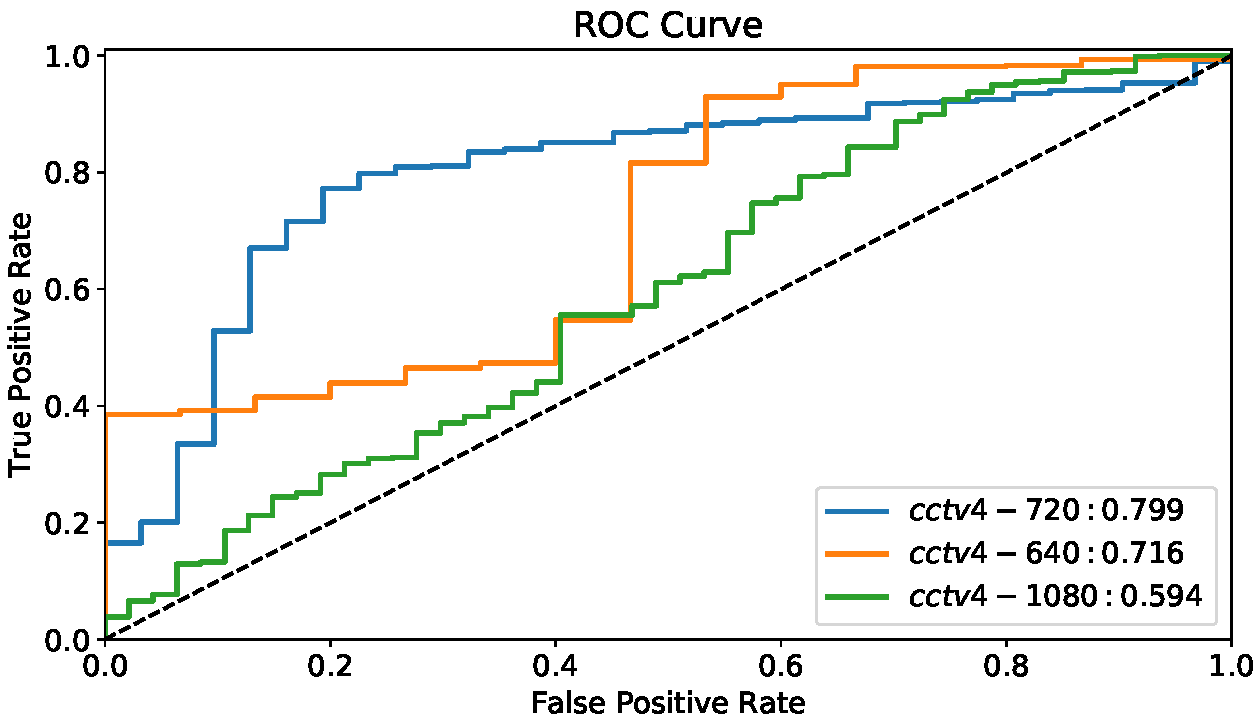
\includegraphics[width=16cm]{figures/roc2.pdf}
\caption{ROC křivky klasifikátoru konfigurace 15 na videosekvencích z~tabulky \ref{videosTab}}
\label{fig:rocCurve2}
\end{figure}

Předfiltrování obrazu pomocí subtrakce pozadí se značně projevilo při detekci chodců. Nejen, že se zefektivnila detekce odfiltrováním většiny false positive detekcí, ale také rychlost samotného detektoru. Například na dvoujádrovém počítači Banana Pi je rychlost skoro až $7\times$ rychlejší než se samotnou metodou HOG při nízkém rozlišení videa (cctv04\_640).

Nejvhodnějším zařízením pro detekování chodců při této implementaci se projevil Raspberry PI. Navzdory optimalizování algoritmu nelze hovořit o~úspěchu, protože touto implementací nelze detekovat chodce v~reálném čase.